\section{Zyklische Belastung}
    \subsection{Ermüdung}
        Progressive Shädigiung durch zyklische Belastung $\rightarrow$ Riss $\rightarrow$ Dauerbruch\\
        Einflüsse: 3D Spannungszustand, Temp., Korr., Zeit, Frequenz d Zyklen, Kerbwirkung, Mittelspannung, Eigenspannungen, Kumulative Ermüdung, Oberfläche
        \subsubsection{Allgemeines Vorgehen}
            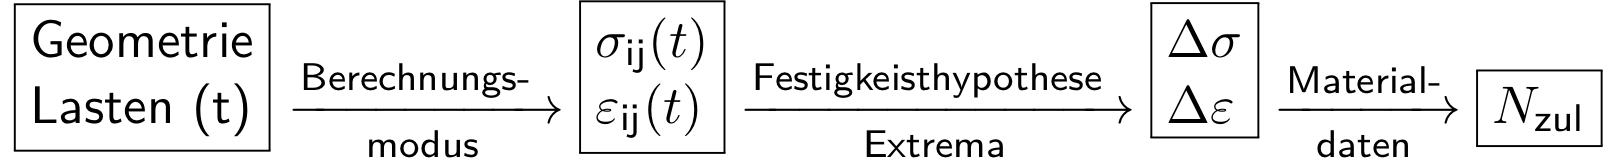
\includegraphics[width=\linewidth]{06/allg_vorgehen.jpeg}
        \subsection{Dauer- \& Zeitfestigkeit}
            \begin{minipage}{\linewidth}
                \begin{itemize}
                    \item bis $10^3-10^4$ Zyklen: LCF (low cycle fatigue - Kurzzeitfestigkeit)
                    \item $10^3-10^4$ bis $10^6$: HCF (high cycle fatigue - Langzeitfestigkeit)
                    \item ab $10^6-10^7$: Dauerfestigkeit - $\sigma_W$: Wechselfestigkeit
                \end{itemize}
            \end{minipage}
    \subsection{Einfluss der Mittelspannung aud Dauerfestigkeit}
        \[\sigma_m=\frac{\sigma_u+\sigma_o}{2}; \quad R=\frac{\sigma_u}{\sigma_o} \quad \sigma_m \uparrow, R \uparrow (\sigma_o >0) \rightarrow N_{zul} \downarrow\]
        \begin{center}
            \vspace{-2mm}
            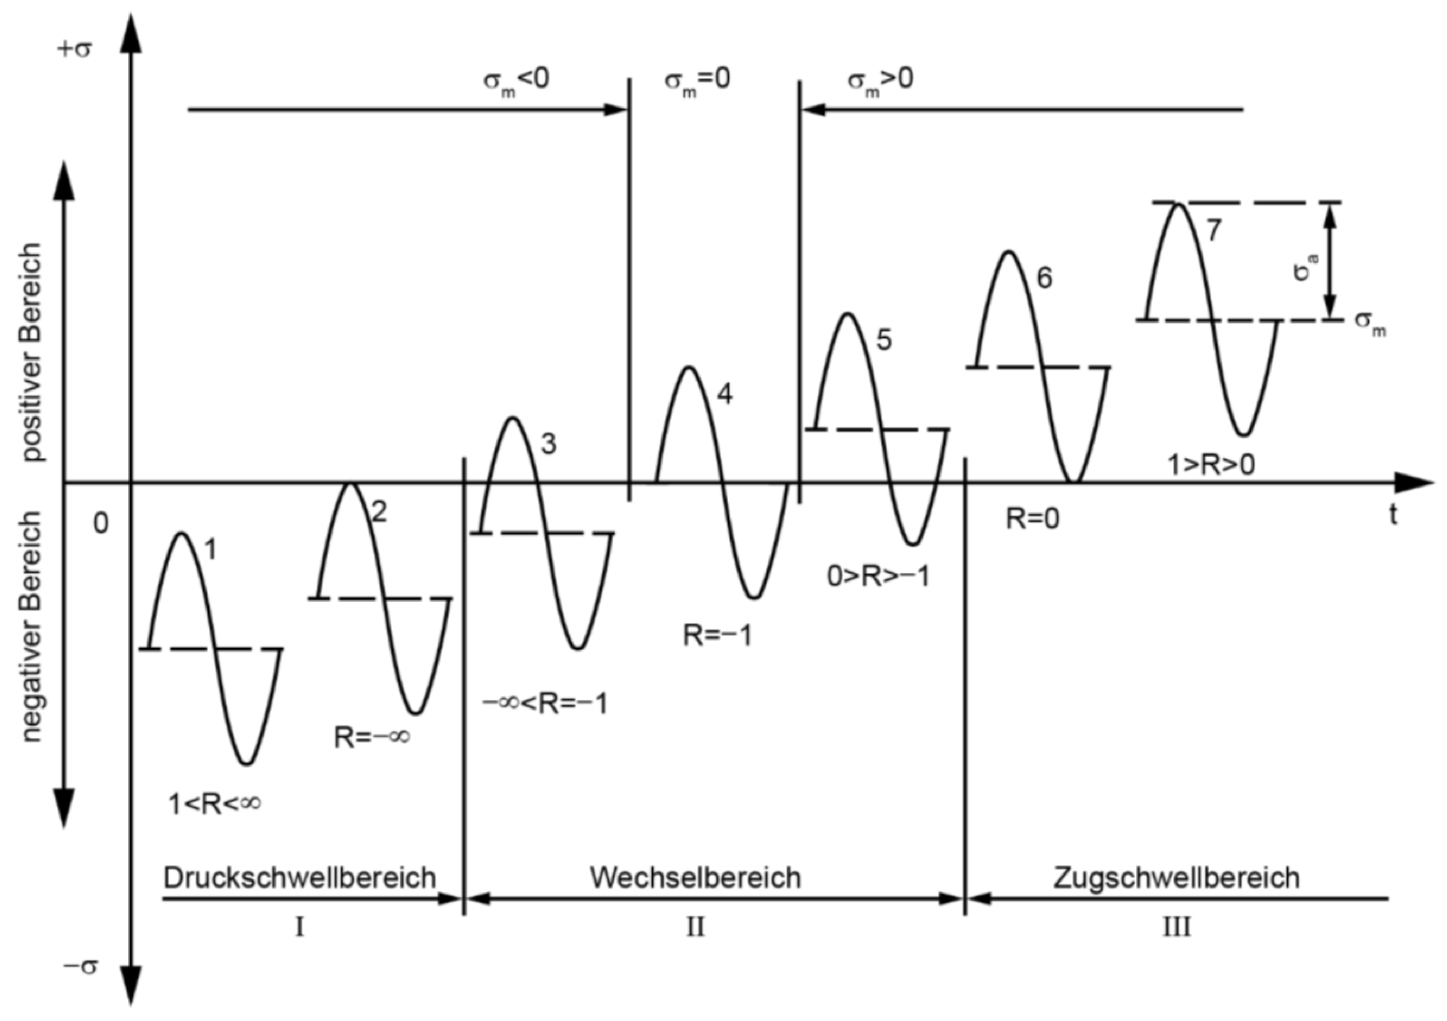
\includegraphics[width=0.8\linewidth, height= 35mm]{06/Einfluss_mittelspannung.png}
        \end{center}
    \subsection{Smith-Diagram}
        
        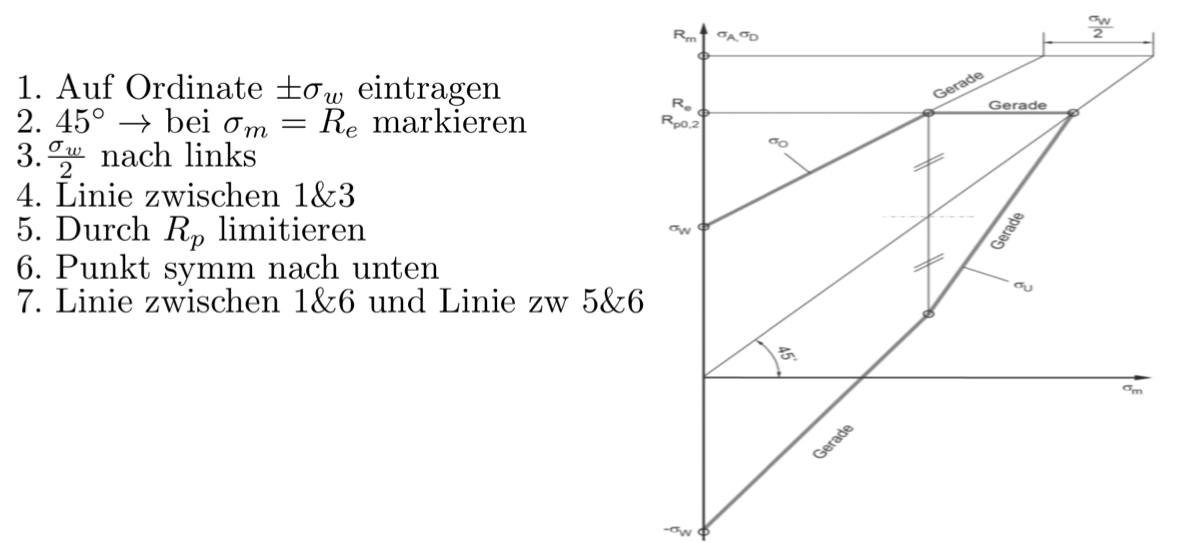
\includegraphics[width=\linewidth, height= 40mm]{06/smith_diagramm.jpeg}
    \subsection{Kumulative Ermüdung}
        Belastung oft komplexer als 'einstufig' $\rightarrow$ Mehrstufenkollektiv. Belastungsfunktion wird in Abschnitte aufgeteilt.
        \[D_{\textrm{BK}}= \sum_{i}\frac{n_{i}}{N_{\textrm{Zul}}(\Delta\sigma_{i},\sigma_{m,i})} \quad D_{\textrm{BK}}: \frac{\textrm{Schädigung}}{\textrm{Belastungskollektive}} \]
        \[T_{L}=\frac{1}{D_{\textrm{BK}}}\cdot T_{\textrm{BK}} \quad\quad\quad T_{\textrm{BK}}:\frac{\textrm{Belastungszeit}}{\textrm{Belastungskollektive}}\]
    \subsection{Kerben}
        \subsubsection{Lokal Elastisch}
            Anriss erfolgt oft an Kerben. An der kritischen Stelle oft \textbf{Ebener Spannungszustand} (Spannungsfreie Oberfläche).\\ $K_F$: Abminderung der Zeitfestigkeit; $K_T$: Abminderung der Wechselfestigkeit. Da $K_F < K_T$ wäre eine Beurteilung basierend auf der lokalen Spannungsamplitude mit der Wöhlerkurve aus ungekerbten Proben zu konservativ. $\sigma_{\textrm{max}}=K_F \cdot \sigma_{\textrm{nom}}$ statt $K_T$.
            \[K_F = q\cdot(K_T-1)+1\]
        \subsubsection{Lokal inelastisch}
            LCF an Kerbe.
            \[\Delta\sigma_K = K_{\sigma} \cdot \Delta\textrm{s} \quad\quad \Delta\textrm{s}:\textrm{Fernfeld Schwingbreite}\]
            \[\Delta\varepsilon_K = K_{\varepsilon} \cdot \Delta\textrm{e} \quad\quad \Delta\sigma_K:\textrm{lok. Schwingbreite}\]
            \[\Delta\textrm{e}=\frac{\Delta s}{E} \quad\quad\quad \Delta\varepsilon_K:\textrm{lok. Schwingbreite}\]
    \subsection{Neuber Hyperbel}
        \TODO{}
    \subsection{BSP}
        \TODO{BSP VON SERIE}
    
    